\chapter{THIẾT KẾ GIẢI PHÁP VÀ HIỆN THỰC ỨNG DỤNG}
\label{chap:4-design}

% TODO: đoạn dẫn nhập chương

\section{Kiến trúc tổng thể}
\label{sec:4-architecture}
% TODO

\section{Công nghệ quản lý dữ liệu}
\label{sec:4-storage}
% TODO

\section{Công nghệ xử lý dữ liệu}
\label{sec:4-processing}
% TODO

\section{Thiết kế mô hình dữ liệu}
\label{sec:4-data-model}
% TODO: các tầng dữ liệu (thô, đã làm sạch, tổng hợp)

\section{Pipeline micro-batch theo từng yêu cầu nghiệp vụ}
\label{sec:4-pipeline}

\subsection{BR01 -- Tập trung hóa giám sát nông nghiệp}
\subsection{BR02 -- Nâng cao nhận biết điều kiện đồng ruộng}
\subsection{BR03 -- Duy trì tính liên tục của giám sát}
\subsection{BR04 -- Thiết lập dữ liệu đáng tin cậy}
\label{sec:4-br04}

\paragraph{Yêu cầu.} Người dùng không được ra quyết định dựa trên số đo sai, trùng hoặc gây hiểu nhầm, và mọi con số phải truy ngược được về nguồn (FR4.1--FR4.7).

\paragraph{Luồng dữ liệu.} Việc bảo đảm chất lượng được đặt ở hai nơi. Kiểm định chạy \emph{trong} mỗi micro-batch của Spark, nên dữ liệu lỗi bị chặn trước khi tới bảng điều khiển gần thời gian thực. Tổng hợp và kiểm thử chạy \emph{sau} trong dbt, nên tầng gold chỉ được làm mới khi dữ liệu đạt các test. Hình~\ref{fig:4-br04-flow} mô tả luồng này.

\begin{figure}[H]
\centering
\begin{tikzpicture}[
  node distance=0.45cm and 0.5cm,
  box/.style={rectangle, rounded corners, draw, minimum width=2.2cm, minimum height=0.9cm, align=center, font=\footnotesize, fill=gray!10},
  ok/.style={box, fill=green!10}, bad/.style={box, fill=red!10},
  arr/.style={-{Stealth}, thick}]
\node[box, fill=blue!10] (k) {Kafka\\sự kiện thô};
\node[box, right=of k] (s) {Schema\\tường minh};
\node[box, right=of s] (r) {Gán thiết bị\\vào thửa ruộng};
\node[bad, below=of r] (q) {ops.quarantine\\(lý do + payload)};
\node[box, right=of r] (f) {Gắn cờ: trùng,\\rỗng, ngoài khoảng,\\bước nhảy};
\node[ok, below=of f] (b) {bronze\\(có cờ, có lineage)};
\node[box, below=of b] (c) {ops.quality\_counters};
\node[ok, left=of c] (sv) {silver (dbt)\\+ test};
\node[ok, left=of sv] (g) {gold quality\_daily};
\draw[arr] (k)--(s); \draw[arr] (s)--(r); \draw[arr] (r)--(f);
\draw[arr] (r)--node[left, font=\scriptsize]{lỗi cấu trúc}(q);
\draw[arr] (f)--(b); \draw[arr] (f.east) to[bend left=40] (c.east);
\draw[arr] (b)--(sv); \draw[arr] (c)--(sv); \draw[arr] (sv)--(g);
\end{tikzpicture}
\caption{Luồng bảo đảm chất lượng dữ liệu của BR04}
\label{fig:4-br04-flow}
\end{figure}

\paragraph{Bước 1: schema tường minh (FR4.1).} Tác vụ không suy diễn schema. Mọi trường của payload được đọc dưới dạng chuỗi, để phân biệt được hai trường hợp: giá trị sai kiểu (ví dụ \code{"value": "high"}) là lỗi cấu trúc và bị cách ly, còn giá trị \code{null} hợp lệ về JSON là một số đo rỗng và chỉ bị gắn cờ.

\begin{lstlisting}[language=Python, caption={Schema tường minh của payload (\texttt{src/streaming/config.py})}, label={lst:4-payload-schema}]
PAYLOAD_COLUMNS = {
    "event_id": "string", "device_id": "string", "metric": "string",
    "value": "string", "reading_ts": "string",
    "battery_pct": "string", "signal_quality": "string",
    "simulated_fault": "string",
}
schema = StructType([StructField(n, StringType(), True) for n in PAYLOAD_COLUMNS])
\end{lstlisting}

\paragraph{Bước 2: cách ly lỗi cấu trúc.} Mỗi bản ghi được gán một lý do cách ly theo thứ tự ưu tiên ở Đoạn mã~\ref{lst:4-quarantine-reason}. Bản ghi có lý do khác rỗng đi vào \code{ops.quarantine}; phần còn lại đi tiếp. Nhờ vậy một payload hỏng không làm dừng cả micro-batch.

\begin{lstlisting}[language=Python, caption={Lý do cách ly (\texttt{src/streaming/pipeline.py}, \texttt{\_stage})}, label={lst:4-quarantine-reason}]
reason = (
    F.when(~F.col("json_ok"), F.lit("invalid_json"))
    .when(blank_device | blank_metric | blank_ts, F.lit("missing_field"))
    .when(F.col("measured_at").isNull(), F.lit("invalid_timestamp"))
    .when(F.col("value_raw").isNotNull() & value.isNull(), F.lit("malformed_value"))
    .when(F.col("resolved_field_id").isNull(), F.lit("unknown_device"))
    .when(~F.array_contains(device_metrics[F.col("device_id")], F.col("metric")),
          F.lit("unexpected_metric"))
    .otherwise(F.lit(None).cast("string"))
)
\end{lstlisting}

\paragraph{Bước 3: gắn cờ chất lượng (FR4.2, FR4.3).} Với các bản ghi hợp lệ về cấu trúc, cờ \code{quality\_flag} nhận một trong năm giá trị: \code{duplicate}, \code{null\_value}, \code{out\_of\_range}, \code{implausible\_jump} hoặc \code{ok}. Ngưỡng của từng chỉ số nằm trong dữ liệu danh mục (Bảng~\ref{tab:4-metric-ranges}), nên đổi ngưỡng không cần sửa mã. Bước nhảy được so với giá trị mới nhất của cùng thửa ruộng và chỉ số trong Cassandra.

\begin{table}[H]
\centering
\caption{Ngưỡng kiểm định theo chỉ số (\texttt{reference/reference\_data.json})}
\label{tab:4-metric-ranges}
\small
\begin{tblr}{
  colspec = {X[2,l]X[1,c]X[1,c]X[1,c]X[1.4,c]}, rows = {abovesep=2pt, belowsep=2pt},
  hlines, vlines, row{1} = {font=\bfseries, bg=gray!20},
}
Chỉ số & Đơn vị & Nhỏ nhất & Lớn nhất & Bước nhảy tối đa \\
soil\_moisture & \% & 0 & 100 & 25 \\
soil\_temperature & $^\circ$C & $-10$ & 50 & 12 \\
air\_temperature & $^\circ$C & $-30$ & 60 & 15 \\
relative\_humidity & \% & 0 & 100 & 30 \\
rainfall & mm/h & 0 & 200 & 40 \\
\end{tblr}
\end{table}

\paragraph{Bước 4: ghi bronze, bảng đếm và lineage (FR4.4, FR4.5).} Bản ghi được ghi vào bronze bằng \code{MERGE} theo khóa \code{(device\_id, metric, measured\_at)}, kèm sáu cột lineage. Đồng thời mỗi lô ghi một dòng đếm cho mỗi cặp thiết bị và chỉ số vào \code{ops.quality\_counters} (tổng, hợp lệ, trùng, rỗng, ngoài khoảng, bước nhảy, đến muộn). Bảng đếm này là nguồn của báo cáo chất lượng hằng ngày.

\paragraph{Bước 5: dbt và tầng gold (FR4.5, FR4.7).} Model silver khử trùng lặp lần thứ hai (Đoạn mã~\ref{lst:2-silver}) và mang các test ở Đoạn mã~\ref{lst:2-silver-tests}. Model gold \code{quality\_daily} cộng bảng đếm theo ngày và ghép với số bản ghi bị cách ly:

\begin{lstlisting}[language=SQL, caption={Model gold tóm tắt chất lượng (\texttt{dbt/models/gold/quality\_daily.sql}, rút gọn)}, label={lst:4-quality-daily}]
with counters as (
    select cast(date_trunc('day', window_start) as date) as day,
           sum(total) as total, sum(valid) as valid,
           sum(duplicate) as duplicate, sum(out_of_range) as out_of_range,
           sum(null_value) as quarantined
    from {{ source('ops', 'quality_counters') }} group by 1
),
quarantine as (
    select cast(date_trunc('day', detected_at) as date) as day,
           count(*) as quarantined
    from {{ source('ops', 'quarantine') }} group by 1
)
select c.day, c.valid, c.duplicate, c.out_of_range,
       coalesce(q.quarantined, c.quarantined, 0) as quarantined, c.total
from counters c left join quarantine q on q.day = c.day
\end{lstlisting}

Cột \code{quarantined} lấy số bản ghi bị cách ly trong ngày; nếu ngày đó không có bản ghi cách ly nào, model dùng số bản ghi rỗng (\code{null\_value}) thay thế. Hai khái niệm này khác nhau (bản ghi rỗng vẫn nằm trong bronze), nên Mục~\ref{sec:5-correctness} đối chiếu chúng riêng.

\paragraph{Bước 6: hiển thị (FR4.6).} FastAPI đọc \code{quality\_daily} và bảng silver qua Trino cho trang \emph{Data quality}, gồm biểu đồ theo ngày và bảng theo thiết bị có xem lineage. Trên đường gần thời gian thực, mỗi giá trị trả về kèm \code{quality\_flag} để giao diện đánh dấu điểm đáng ngờ.

\begin{figure}[H]
\centering
\begin{subfigure}[t]{0.48\linewidth}
\centering
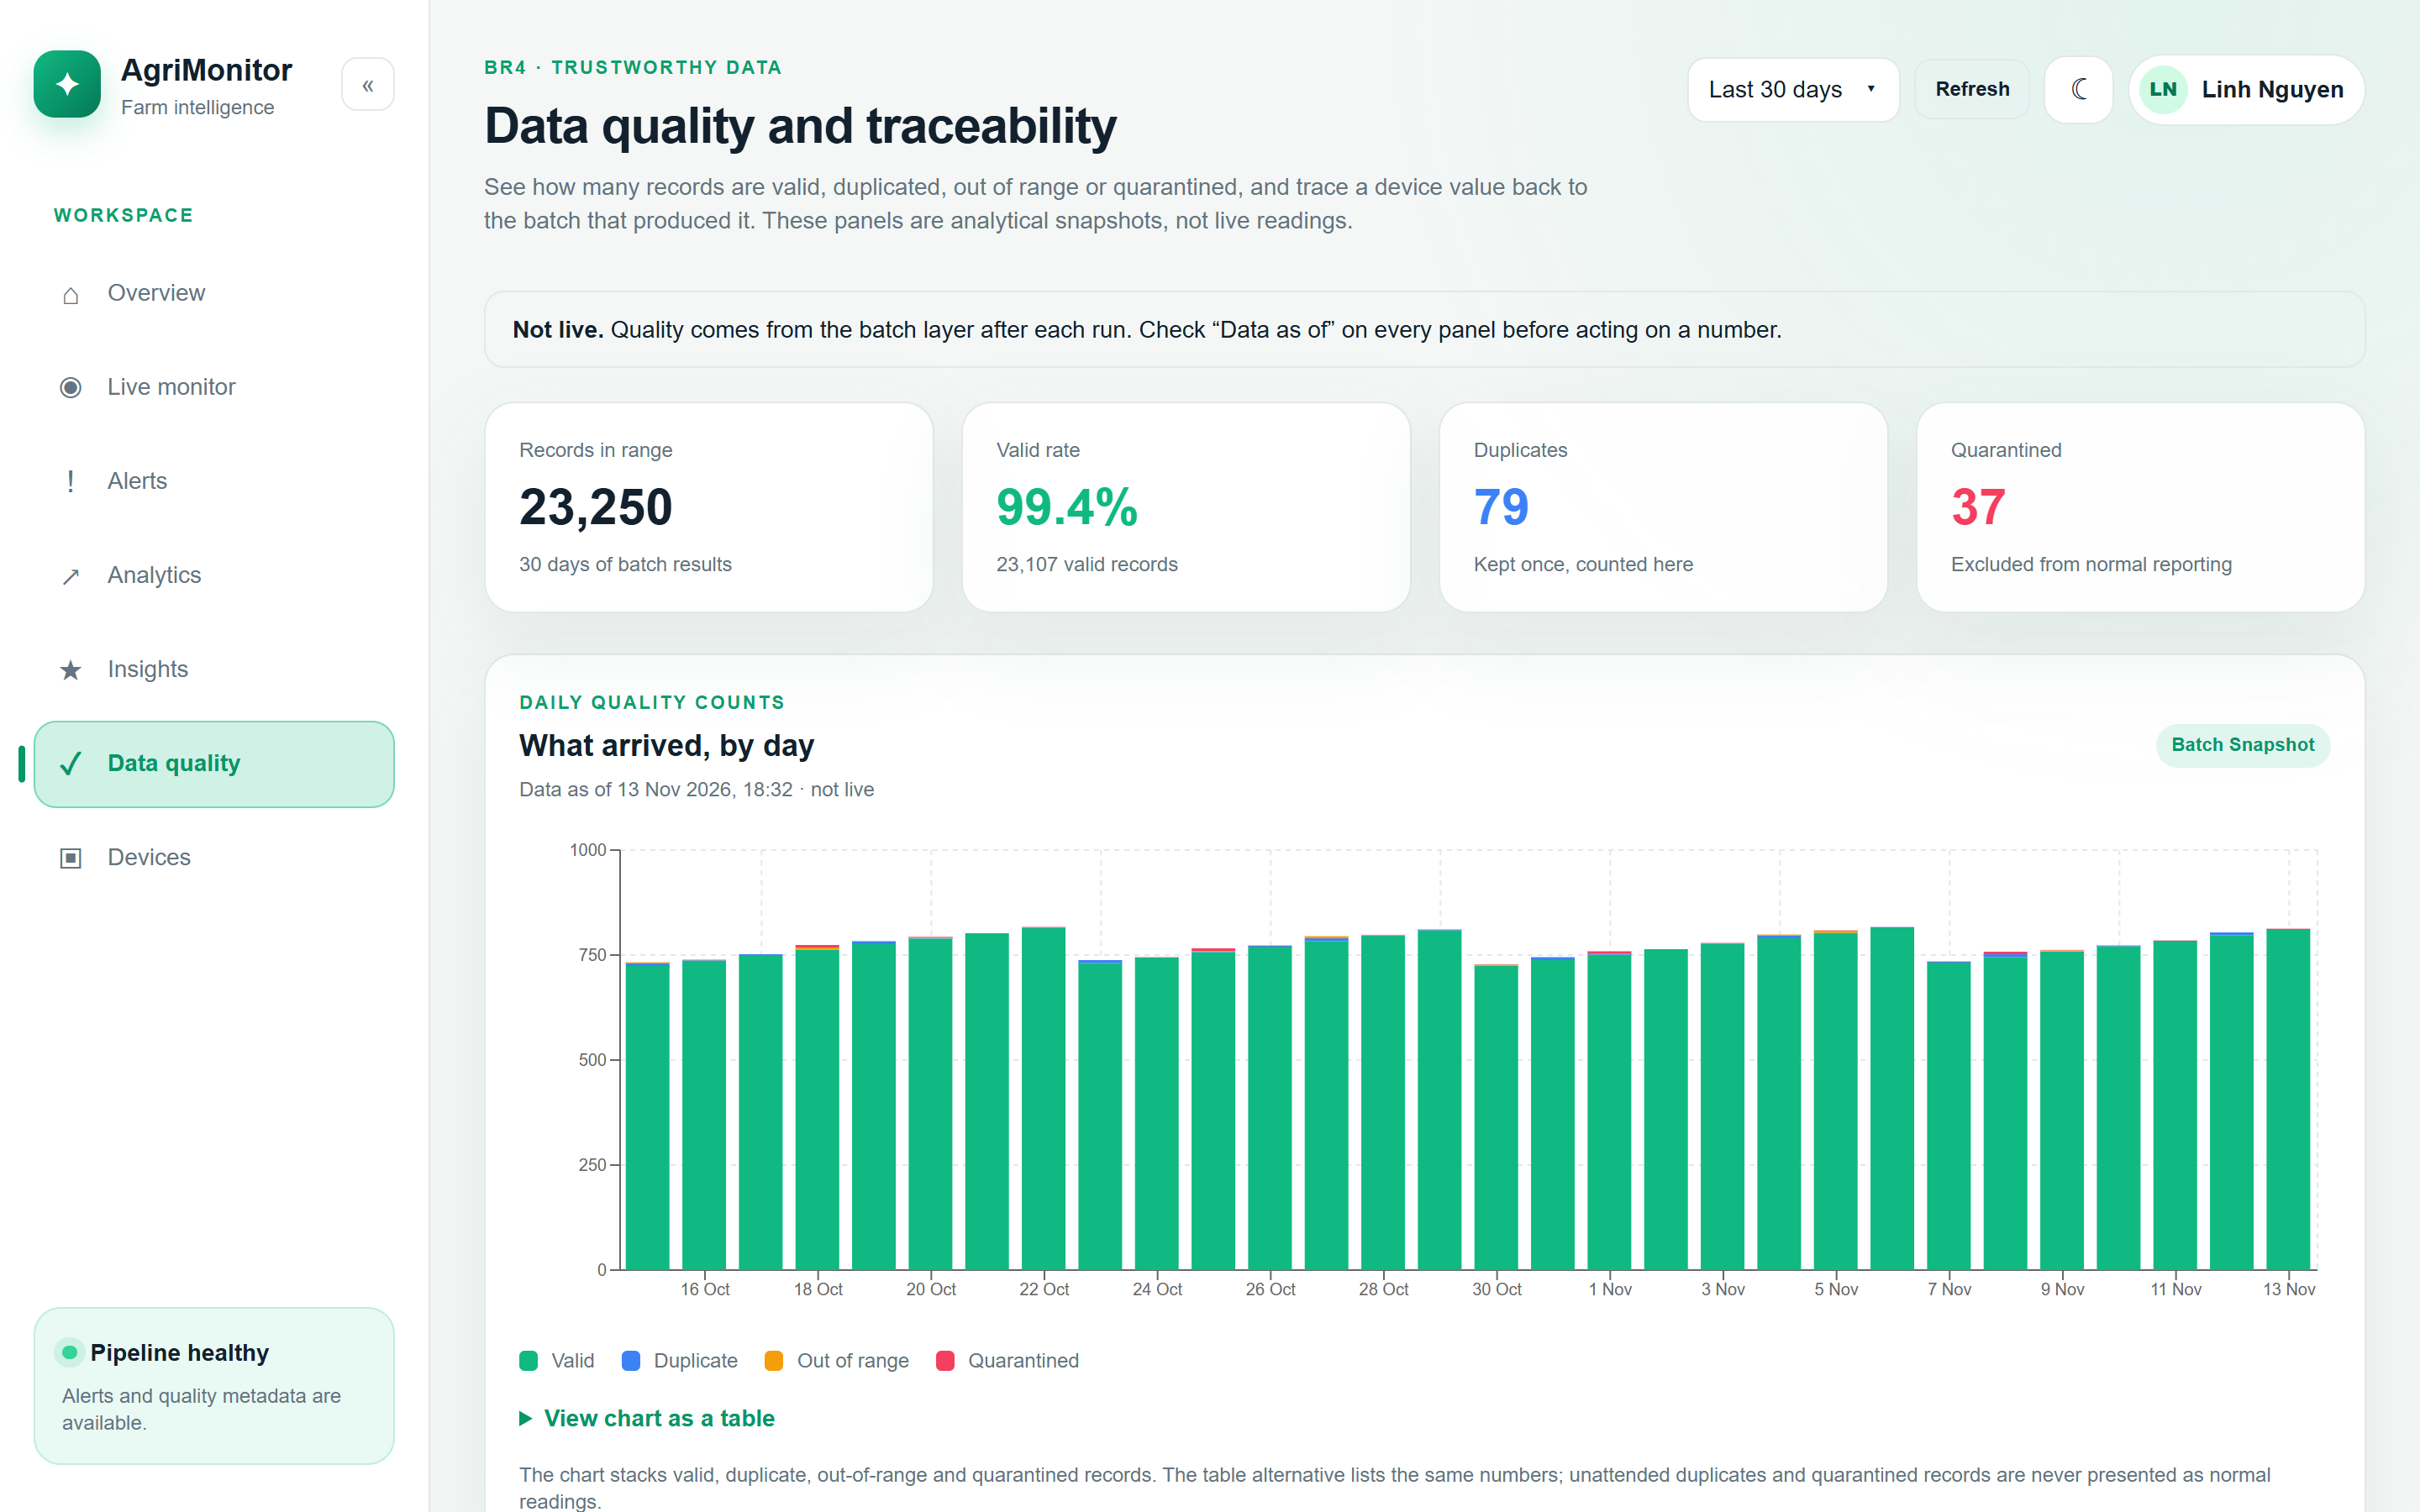
\includegraphics[width=\linewidth]{img/app/quality-chart.png}
\caption{Biểu đồ số bản ghi theo ngày}
\end{subfigure}\hfill
\begin{subfigure}[t]{0.48\linewidth}
\centering
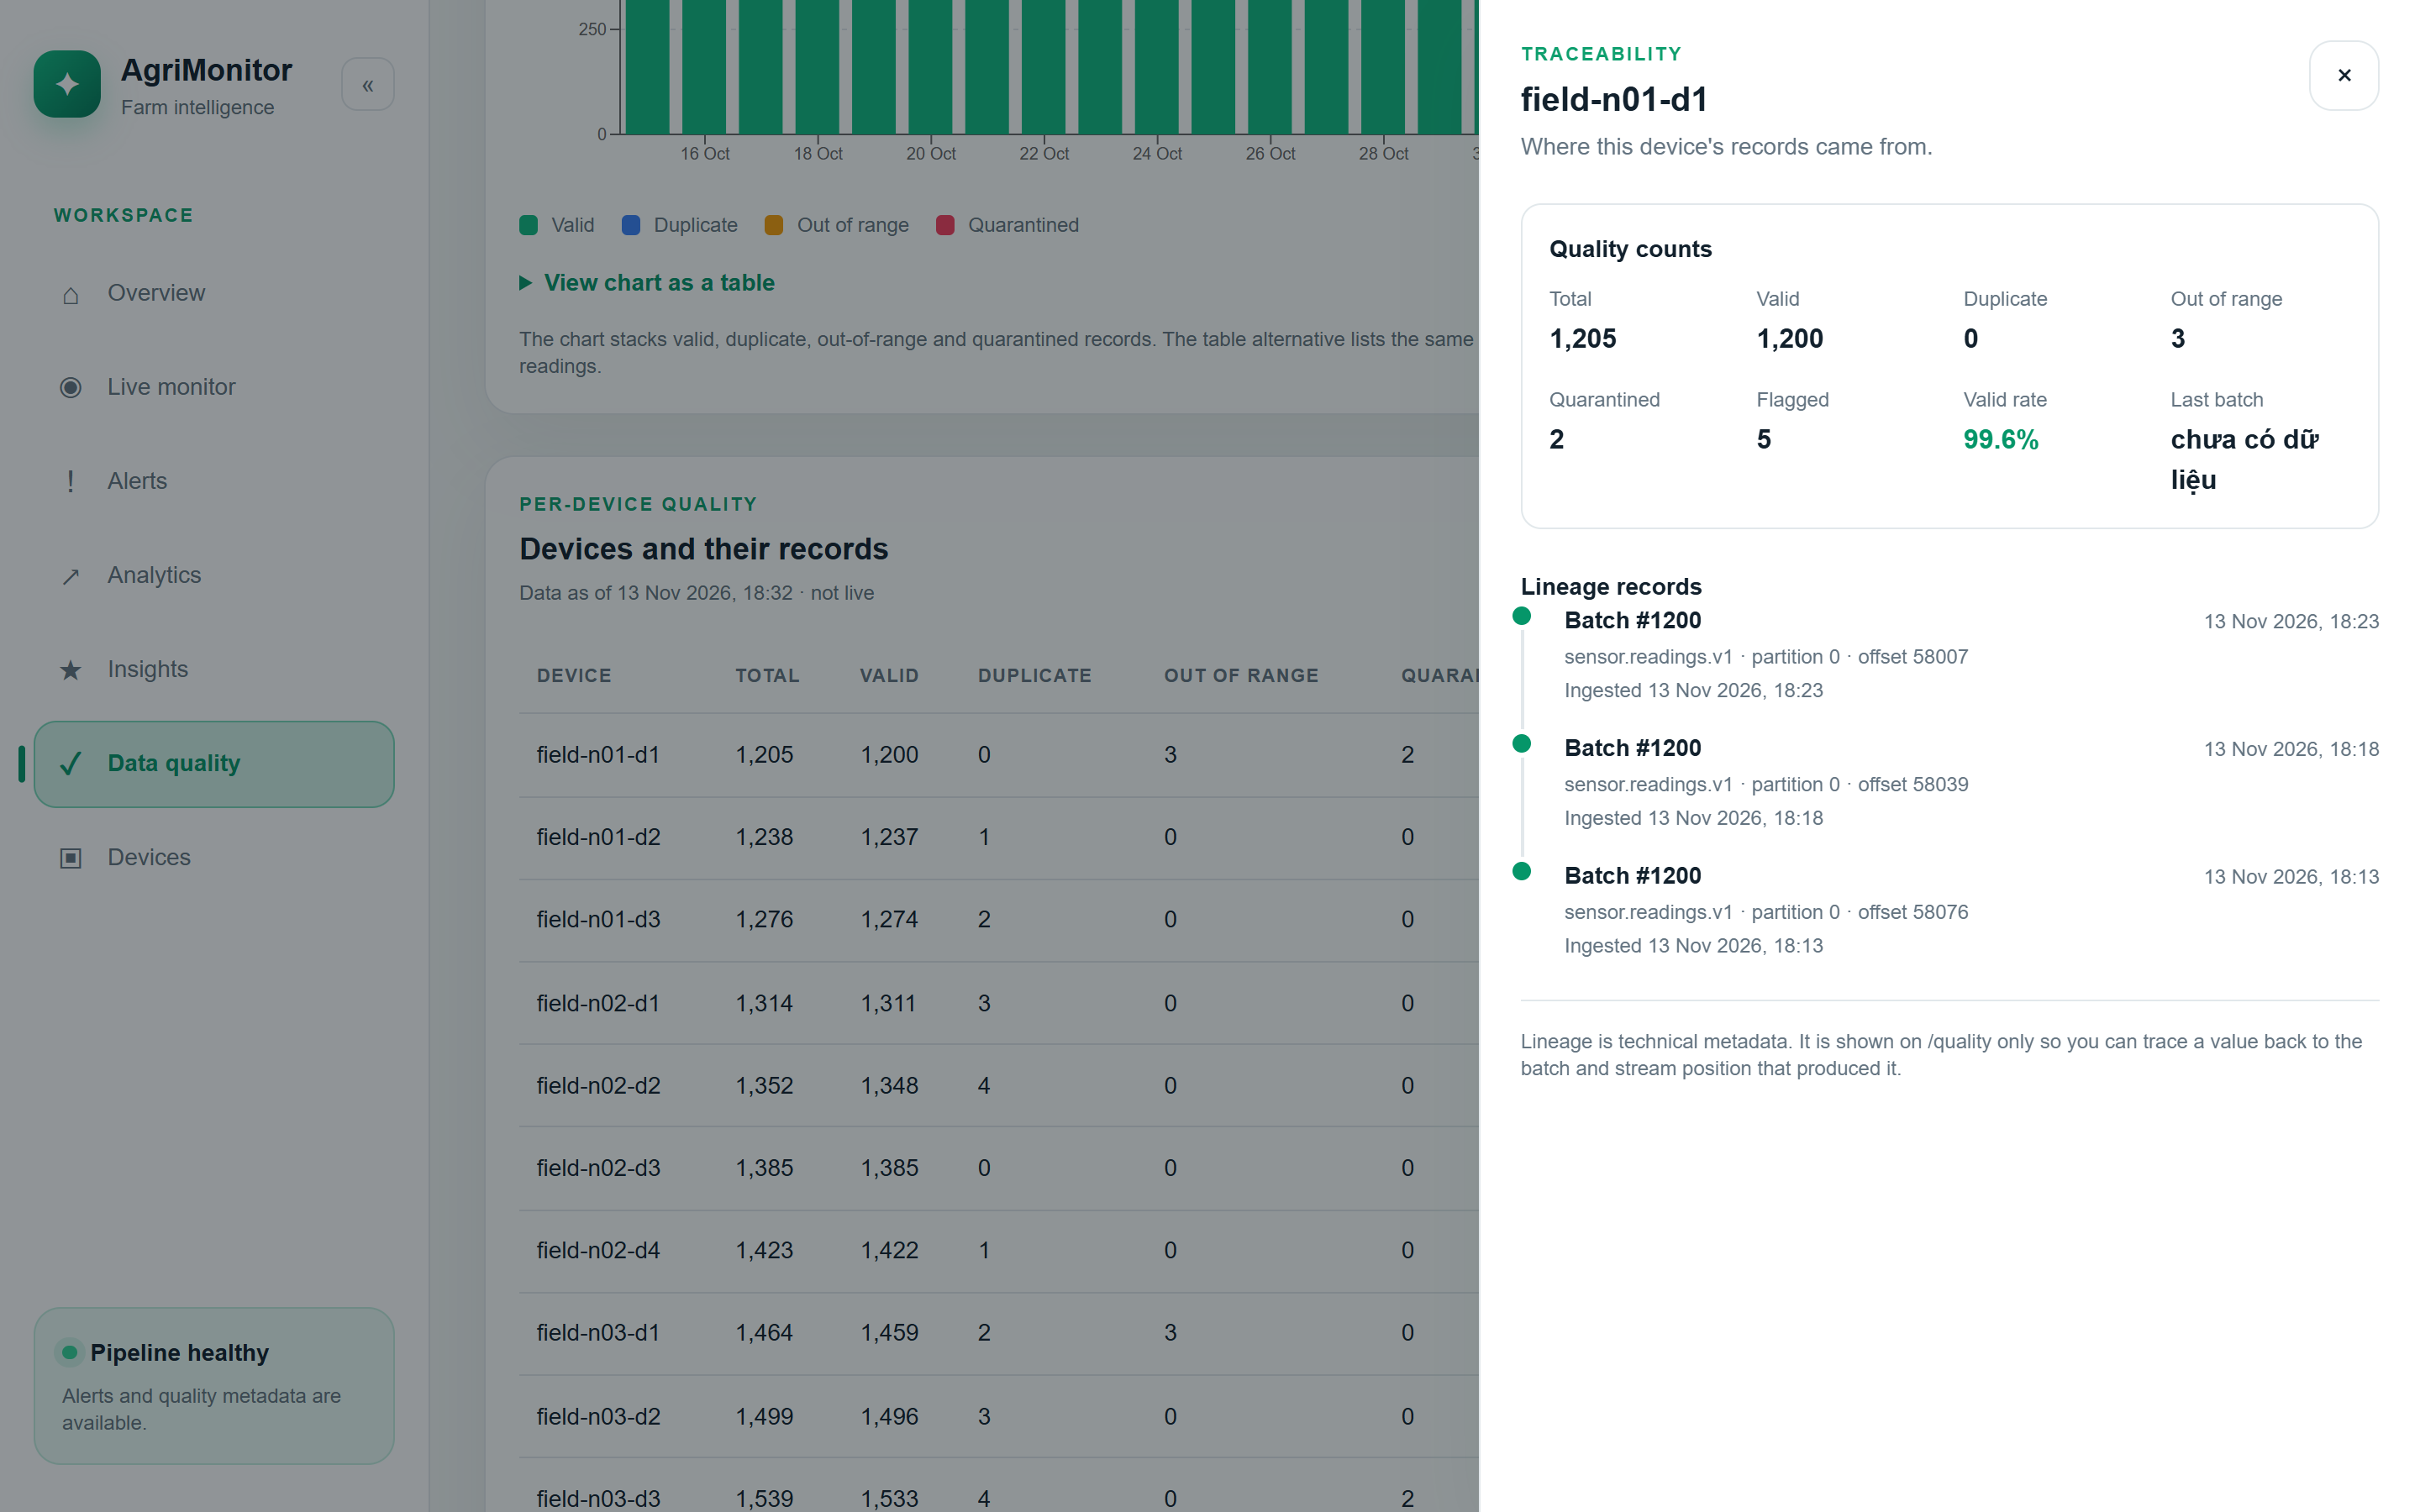
\includegraphics[width=\linewidth]{img/app/quality-lineage.png}
\caption{Lineage của một thiết bị}
\end{subfigure}
\caption{Trang chất lượng dữ liệu của ứng dụng (ảnh chụp với dữ liệu mô phỏng của chế độ \code{DATA\_MODE=mock}).}
\label{fig:4-br04-ui}
\end{figure}

\paragraph{Kết quả và hạn chế hiện tại.} Mọi bản ghi lỗi đều được giữ lại với lý do hoặc cờ, và mọi dòng mang lineage. Có hai điểm còn phải sửa trước khi đánh giá ở Chương~\ref{chap:5-evaluation}. Thứ nhất, model gold \code{field\_daily} hiện tính min, max và trung bình trên mọi giá trị khác rỗng, kể cả dòng có cờ \code{out\_of\_range}; cần giới hạn ở \code{quality\_flag = 'ok'}. Thứ hai, các model gold mới chỉ có test \code{not\_null}; cần thêm test khoảng giá trị (accepted range) để FR4.7 có tác dụng ở tầng gold.

\subsection{BR05 -- Hỗ trợ quản lý dựa trên dữ liệu}
\subsection{BR06 -- Đánh giá lịch sử và lập kế hoạch}
\subsection{BR07 -- Làm cho thông tin dễ tiếp cận}
\subsection{BR08 -- Hỗ trợ ứng phó sớm với rủi ro}
\label{sec:4-br08}

\paragraph{Yêu cầu.} Vận hành viên cần biết sớm khi thửa ruộng có điều kiện bất thường hoặc thiết bị mất kết nối, ghi lại việc mình đã xử lý, và không bị ngập trong cảnh báo lặp lại (FR8.1--FR8.6).

\paragraph{Luồng dữ liệu.} Luật cảnh báo chạy ở cuối mỗi micro-batch, sau khi dữ liệu đã được kiểm định (Mục~\ref{sec:4-br04}). Mỗi lô sinh ra một danh sách \emph{điều kiện} (condition). Mỗi điều kiện đi qua một máy trạng thái có debounce và cooldown, rồi được ghi vào các bảng cảnh báo trong Cassandra. FastAPI đọc các bảng này và nhận thao tác acknowledge hoặc resolve từ vận hành viên.

\subsubsection{Các loại điều kiện}

Bảng~\ref{tab:4-alert-conditions} liệt kê các điều kiện được đánh giá trên mỗi lô. Ngưỡng theo cây trồng nằm trong dữ liệu danh mục; ngưỡng thiết bị lấy từ biến môi trường.

\begin{table}[H]
\centering
\caption{Các điều kiện cảnh báo (\texttt{src/streaming/pipeline.py}, \texttt{\_build\_conditions})}
\label{tab:4-alert-conditions}
\small
\begin{tblr}{
  colspec = {X[1.6,l]X[3,l]X[1,l]X[1,l]}, rows = {abovesep=2pt, belowsep=2pt},
  hlines, vlines, row{1} = {font=\bfseries, bg=gray!20},
}
Điều kiện & Khi nào vi phạm & Mức độ & FR \\
Dưới ngưỡng cây trồng (\code{low\_soil\_moisture}, \ldots) & Trung bình các giá trị \code{ok} trong lô nhỏ hơn \code{alert\_below} của cây trồng & warning & FR8.1 \\
Trên ngưỡng (\code{heat\_stress}, \ldots) & Trung bình lớn hơn \code{alert\_above} & critical & FR8.1 \\
Thay đổi đột ngột (\code{rapid\_change}) & Có bản ghi cờ \code{implausible\_jump} & info & FR8.1 \\
Mất kết nối (\code{device\_offline}) & Thiết bị im lặng lâu hơn 4 lần chu kỳ báo cáo & warning & FR8.2 \\
Pin yếu (\code{battery\_low}) & Pin $\le$ 20\% & warning & FR8.2 \\
Sóng yếu (\code{signal\_poor}) & Chất lượng tín hiệu $<$ 0,3 & info & FR8.2 \\
\end{tblr}
\end{table}

Ví dụ với lúa (\code{RICE}): khoảng độ ẩm đất mục tiêu là 30--60\% và ngưỡng cảnh báo \code{alert\_below} là 32\%. Nếu trung bình độ ẩm các bản ghi hợp lệ trong một lô của thửa F001 là 29,5\%, điều kiện \code{low\_soil\_moisture} của F001 ở trạng thái vi phạm.

Điều kiện mất kết nối được đánh giá cho \emph{mọi} thiết bị trong danh mục ở mỗi lô, kể cả khi lô không có dữ liệu. Để Spark vẫn chạy lô khi Kafka im lặng hoàn toàn, nguồn Kafka được hợp (\code{unionByName}) với nguồn \code{rate} của Spark phát một dòng nhịp mỗi giây; các dòng nhịp bị lọc bỏ ngay sau đó. Nếu thiếu cơ chế này, sự cố mất kết nối toàn bộ sẽ không bao giờ được phát hiện vì không có lô nào chạy.

\subsubsection{Máy trạng thái: debounce, cooldown và tự đóng}

Toàn bộ logic quyết định nằm trong một hàm thuần Python, không phụ thuộc Spark hay Cassandra, nên kiểm thử đơn vị được (Đoạn mã~\ref{lst:4-evaluate}).

\begin{lstlisting}[language=Python, caption={Máy trạng thái cảnh báo (\texttt{src/streaming/alerts.py}, rút gọn)}, label={lst:4-evaluate}]
def evaluate(condition, state, now, cfg) -> Decision:
    if condition.breaching:
        state.debounce_count += 1
        if state.open_alert_id is not None:          # already open
            return Decision(emit_alert=False, resolve_alert=False)
        if state.debounce_count < cfg.debounce_batches:   # debounce
            return Decision(emit_alert=False, resolve_alert=False)
        if state.last_emitted_at is not None and \
           (now - state.last_emitted_at).total_seconds() < cfg.cooldown_s:
            return Decision(emit_alert=False, resolve_alert=False)  # cooldown
        return Decision(emit_alert=True, resolve_alert=False)
    state.debounce_count = 0                           # condition cleared
    if state.open_alert_id is not None and state.open_status == "open":
        return Decision(emit_alert=False, resolve_alert=True)    # auto-resolve
    return Decision(emit_alert=False, resolve_alert=False)
\end{lstlisting}

Ba quy tắc chống bão cảnh báo (FR8.5) và vòng đời (FR8.4) như sau:

\begin{itemize}
  \item \textbf{Debounce}: điều kiện phải vi phạm liên tiếp \code{ALERT\_DEBOUNCE\_BATCHES} lô (mặc định 2) mới sinh cảnh báo, nên một lô nhiễu không gây cảnh báo. Với trigger 30 giây, cảnh báo xuất hiện sau khoảng 60 giây kể từ lô vi phạm đầu tiên.
  \item \textbf{Một cảnh báo cho một sự cố}: khi đã có cảnh báo mở cho điều kiện đó, các lô vi phạm tiếp theo không sinh thêm cảnh báo.
  \item \textbf{Cooldown}: sau khi một cảnh báo được phát, cùng điều kiện không được phát lại trong \code{ALERT\_COOLDOWN\_S} giây (mặc định 300).
  \item \textbf{Tự đóng}: khi điều kiện hết vi phạm, cảnh báo đang ở trạng thái \code{open} được đóng tự động với lý do \code{condition\_cleared}. Cảnh báo mất kết nối vì thế tự đóng khi thiết bị gửi dữ liệu trở lại. Cảnh báo đã được \emph{acknowledge} thì không tự đóng, vì đã có người nhận xử lý và phải do họ đóng.
\end{itemize}

Trạng thái của từng cặp (thửa ruộng, điều kiện), gồm bộ đếm debounce, thời điểm phát gần nhất và cảnh báo đang mở, được lưu trong bảng Cassandra \code{alert\_state\_by\_field}. Vì vậy tác vụ không cần toán tử có trạng thái của Spark, và bộ đếm vẫn còn sau khi tác vụ khởi động lại.

\subsubsection{Lưu trữ và vòng đời trong Cassandra}

Cassandra được mô hình hóa theo truy vấn, nên một cảnh báo được ghi vào ba bảng, mỗi bảng phục vụ một câu truy vấn (Bảng~\ref{tab:4-alert-tables}). Lịch sử cảnh báo được giữ 90 ngày.

\begin{table}[H]
\centering
\caption{Các bảng cảnh báo trong Cassandra (\texttt{cassandra/schema.cql})}
\label{tab:4-alert-tables}
\small
\begin{tblr}{
  colspec = {X[1.5,l]X[1.8,l]X[2.6,l]}, rows = {abovesep=2pt, belowsep=2pt},
  hlines, vlines, row{1} = {font=\bfseries, bg=gray!20},
}
Bảng & Khóa chính & Phục vụ truy vấn \\
\code{alerts\_by\_field} & \code{((field\_id), created\_at, alert\_id)} & Lịch sử cảnh báo của một thửa ruộng, mới nhất trước \\
\code{alerts\_by\_status} & \code{((status), created\_at, alert\_id)} & Danh sách cảnh báo đang mở cho bảng điều khiển \\
\code{alert\_by\_id} & \code{((alert\_id))} & Tra cứu một cảnh báo khi acknowledge hoặc resolve \\
\code{alert\_state\_by\_field} & \code{((field\_id), condition\_code)} & Trạng thái debounce và cooldown của tác vụ streaming \\
\end{tblr}
\end{table}

Vì Cassandra không cho cập nhật cột khóa, đổi trạng thái một cảnh báo nghĩa là xóa dòng khỏi phân vùng trạng thái cũ của \code{alerts\_by\_status} và chèn vào phân vùng mới. Bảng \code{alerts\_by\_field} giữ thông tin người xử lý (\code{acknowledged\_by}, \code{resolved\_by}), thời điểm, cách đóng (\code{manual} hoặc \code{condition\_cleared}) và ghi chú, nên lịch sử phản hồi được bảo toàn.

Thao tác của vận hành viên đi qua \code{PATCH /alerts/\{id\}} của FastAPI. API kiểm tra chuyển trạng thái theo cùng bảng \code{ALLOWED\_TRANSITIONS} với tác vụ streaming và trả mã 409 khi chuyển trạng thái không hợp lệ (ví dụ acknowledge một cảnh báo đã đóng):

\begin{lstlisting}[language=Python, caption={Chuyển trạng thái hợp lệ (\texttt{src/streaming/alerts.py})}, label={lst:4-transitions}]
ALLOWED_TRANSITIONS = {
    "open":         {"acknowledged", "resolved"},
    "acknowledged": {"resolved"},
    "resolved":     set(),
}
\end{lstlisting}

\begin{lstlisting}[language=bash, caption={Acknowledge một cảnh báo qua API}, label={lst:4-patch}]
curl -X PATCH http://localhost:8000/alerts/<alert_id> \
     -H "content-type: application/json" \
     -d '{"action": "acknowledge", "actor": "operator-1", "note": "Irrigation valve opened"}'
\end{lstlisting}

\begin{figure}[H]
\centering
\hinhtrong{0.9\linewidth}{6cm}{Trang Alerts: danh sách cảnh báo, bộ lọc và timeline của một cảnh báo}
\caption{Trang cảnh báo của ứng dụng}
\label{fig:4-br08-ui}
\end{figure}

\paragraph{Kiểm thử.} Logic cảnh báo có 7 kiểm thử đơn vị trong \code{tests/unit/test\_alerts.py}: debounce hoãn các lô đầu, một lô nhiễu không mở cảnh báo, cảnh báo đang mở không bị phát lại, điều kiện hết thì cảnh báo tự đóng, cảnh báo đã acknowledge không tự đóng, cooldown chặn cảnh báo thứ hai quá sớm, và bảng chuyển trạng thái. Logic mất kết nối và khoảng trống dữ liệu có 11 kiểm thử trong \code{tests/unit/test\_status.py}. Cả hai chạy bằng \code{just test-unit}, không cần khởi động cụm.


\section{Giải pháp thay thế để so sánh}
\label{sec:4-alternative}
% TODO: ví dụ xử lý batch thuần hoặc stream thuần (Flink)

\section{Hiện thực ứng dụng}
\label{sec:4-application}

\subsection{Mô phỏng và thu thập dữ liệu}
\subsection{Giao diện người dùng}
\subsection{Triển khai và cấu hình}
\label{sec:4-deployment}

Toàn bộ hệ thống chạy trên một máy bằng Docker Compose. Ba nguyên tắc triển khai: (1) mỗi nhóm dịch vụ khởi động được độc lập qua \emph{profile} của Compose; (2) mọi thao tác thường ngày là một \emph{recipe} của công cụ \code{just}; (3) mọi cấu hình đi qua biến môi trường, không có địa chỉ hay mật khẩu nào viết cứng trong mã.

\paragraph{Các profile của Docker Compose.} Bảng~\ref{tab:4-profiles} liệt kê bốn profile trong \code{docker-compose.yml}. Cassandra thuộc cả hai profile \code{processing} và \code{serving}, vì cả tác vụ streaming lẫn API đều cần nó.

\begin{table}[H]
\centering
\caption{Các profile Docker Compose và dịch vụ (\texttt{docker-compose.yml})}
\label{tab:4-profiles}
\small
\begin{tblr}{
  colspec = {X[1,l]X[3,l]X[2.2,l]}, rows = {abovesep=2pt, belowsep=2pt},
  hlines, vlines, row{1} = {font=\bfseries, bg=gray!20},
}
Profile & Dịch vụ & Vai trò \\
\code{core} & namenode, datanode, kafka, ingest, hive-metastore, trino & Lưu trữ, hàng đợi sự kiện, catalog và engine truy vấn \\
\code{processing} & spark-stream, spark-batch, dbt, spark-tests, simulator, cassandra & Xử lý streaming, xử lý theo lô, kiểm thử, sinh dữ liệu \\
\code{serving} & cassandra, cassandra-init, api & Kho phục vụ gần thời gian thực và FastAPI \\
\code{app} & web & Ứng dụng web Next.js \\
\end{tblr}
\end{table}

\paragraph{Phiên bản thành phần.} Bảng~\ref{tab:4-versions} ghi phiên bản các ảnh Docker được dùng. Mục~\ref{sec:5-setup} dùng lại bảng này để mô tả môi trường thực nghiệm.

\begin{table}[H]
\centering
\caption{Phiên bản các thành phần}
\label{tab:4-versions}
\small
\begin{tblr}{
  colspec = {X[2,l]X[1.5,l]X[2,l]X[1.5,l]}, rows = {abovesep=2pt, belowsep=2pt},
  hlines, vlines, row{1} = {font=\bfseries, bg=gray!20},
}
Thành phần & Phiên bản & Thành phần & Phiên bản \\
Apache Hadoop (HDFS) & 3.3.6 & Apache Iceberg & 1.7.1 \\
Apache Kafka (KRaft) & 3.8.0 & Hive Metastore & 3.1.3 \\
Apache Spark & 3.5.3 & Trino & 438 \\
Apache Cassandra & 5.0.3 & Python & 3.11 \\
\end{tblr}
\end{table}

\paragraph{Các recipe \code{just}.} Người dùng không cần nhớ lệnh \code{docker compose} dài. Đoạn mã~\ref{lst:4-just} là trình tự khởi động một phiên demo đầy đủ.

\begin{lstlisting}[language=bash, caption={Trình tự khởi động hệ thống (\texttt{justfile})}, label={lst:4-just}]
just init            # create .env from .env.example (never overwrites)
just doctor          # check just, docker, compose and .env
just up              # core + serving + processing profiles
just run-stream-bg   # Spark micro-batch job, 30 s trigger
just run-simulator   # LoRaWAN-style sensors with fault injection
just batch-run       # lakehouse-init, dbt build, dbt test, compaction
just up-app          # FastAPI + Next.js web app
just verify-pipeline # row counts in Cassandra, bronze and quarantine
\end{lstlisting}

Bảng~\ref{tab:4-recipes} nhóm các recipe theo mục đích.

{\small
\begin{longtblr}[
  caption = {Các recipe \texttt{just} chính},
  label = {tab:4-recipes},
]{
  width = \linewidth,
  rowhead = 1,
  colspec = {X[1.2,l]X[3,l]}, rows = {abovesep=2pt, belowsep=2pt},
  hlines, vlines, row{1} = {font=\bfseries, bg=gray!20},
}
Nhóm & Recipe \\
Vòng đời & \code{up}, \code{up-core}, \code{up-serving}, \code{up-processing}, \code{up-app}, \code{down}, \code{clean}, \code{ps}, \code{logs} \\
Streaming & \code{run-stream}, \code{run-stream-bg}, \code{stop-stream}, \code{streaming-reset} \\
Dữ liệu vào & \code{run-simulator}, \code{sim-for}, \code{ingest-check}, \code{kafka-tail} \\
Theo lô & \code{lakehouse-init}, \code{dbt-run}, \code{dbt-test}, \code{dbt-docs}, \code{compact}, \code{batch-run} \\
Kiểm tra & \code{verify-pipeline}, \code{trino-sql}, \code{api-health}, \code{test}, \code{test-unit}, \code{lint} \\
Benchmark & \code{bench-trigger}, \code{bench-lookups}, \code{bench-storage}, \code{bench-compaction}, \code{bench-replay} \\
\end{longtblr}
}

\paragraph{Cấu hình qua biến môi trường.} Tệp \code{.env.example} là mẫu cấu hình duy nhất; \code{just init} sao chép nó thành \code{.env}, tệp này không được commit. Các tham số của tác vụ streaming được truyền vào container qua khối \code{x-spark-env} của Compose, với giá trị mặc định đặt ngay tại đó (Đoạn mã~\ref{lst:4-env}). Nhờ vậy benchmark có thể đổi chu kỳ trigger mà không sửa mã, ví dụ \code{just run-stream trigger=10s}.

\begin{lstlisting}[caption={Tham số streaming và cảnh báo (\texttt{docker-compose.yml}, khối \texttt{x-spark-env}, rút gọn)}, label={lst:4-env}]
SPARK_DRIVER_MEMORY: ${SPARK_DRIVER_MEMORY:-2g}
TRIGGER_INTERVAL: ${TRIGGER_INTERVAL:-30s}
MAX_OFFSETS_PER_TRIGGER: ${MAX_OFFSETS_PER_TRIGGER:-20000}
WATERMARK_S: ${WATERMARK_S:-3600}
LATE_AFTER_S: ${LATE_AFTER_S:-600}
ALERT_DEBOUNCE_BATCHES: ${ALERT_DEBOUNCE_BATCHES:-2}
ALERT_COOLDOWN_S: ${ALERT_COOLDOWN_S:-300}
DEVICE_OFFLINE_MULTIPLIER: ${DEVICE_OFFLINE_MULTIPLIER:-4}
BATTERY_LOW_PCT: ${BATTERY_LOW_PCT:-20}
SIGNAL_POOR_MAX: ${SIGNAL_POOR_MAX:-0.3}
\end{lstlisting}

\paragraph{Yêu cầu tài nguyên.} Docker cần tối thiểu 8~GB bộ nhớ; 12~GB thoải mái hơn khi HDFS, Kafka, Cassandra, Spark, Trino và Hive Metastore chạy cùng lúc. Spark chạy ở chế độ \code{local[*]} với bộ nhớ driver 2~GB, 4 nhân và 4 phân vùng shuffle, phù hợp khối lượng dữ liệu demo.

